\chapter{Sensor nodes}
\label{chap:nodes}

This chapter will describe functionalities of sensor node devices. After that it will describe how electronic parts were chosen. A separate section will include details regarding \ac{PCB} design while another section will describe software developed for the sensor nodes. Both software and hardware files are available with additional instructions on \href{github.com/Xenosb/thesis-atmel}{GitHub} page.

\section{Physical design and connections}

Most of the required \ac{PCB} features were already described in the previous chapter - board should allow direct connection of \ac{FSR} sensors, it should eliminate need for additional perforated boards and it should provide a more robust solution for physical board position detection. Furthermore, it should feature low power consumption and enable connection of at least two rows of 8 pressure sensors. Also it should feature small dimensions and provide mounting holes so that it doesn't have to be suspended by wires or taped to the bed. The ideal position for the installation of the board is under the bed base slates. This way it can easily be serviced.

There are 4 variants of pin endings found on \ac{FSR} sensors. A variant with no leads is used for custom pin endings while solder tabs variant is used for direct soldering to the board. Because of the materials used for construction of the sensor, when heat is applied using standard soldering iron, there is a high possibility of sensor leads melting. This is why a female plug connector option was chosen. Distance between leads is $1/10"$ and they are compatible with standard \ac{PCB} connector pins. Since sensors will be mounted on pressure disks which are found on the upper side of the bed base, while the board is found under the slates, elongation cables are required. In this case, DuPont 'jumper' cables will be used and a board connectors have been designed in such a way. Two edges of the board, are populated with 8 two-row connectors. Row on the top is connected to the \ac{ADC} pins of the microcontroller while the bottom pins are grounded. In front of each of the pins, a reference resistor $R_{ref}$ is found.

Connector that was used for internal communication bus features 6 wires - 2 wires are used for \ac{I2C}, 2 are used for power supply and 2 are used for physical position recognition. Because they are interchangeable with DuPont jumper wires and because of toolless cable connector installation, \ac{IDC} cables and connectors were used\cite{IDC}. There are two 3x2 internal communication bus connectors on the board so that boards can easily be 'daisy-chained'. Close to the first connector, two pull-down resistors for I2C bus are situated. For microcontroller programming, the same type of connectors was used. The cortex debug interface consists of 10 pins so a single 5x2 connector was used. Graphic \ref{fig:connectors} shows connectors with positions of pins.

\begin{figure}[h]
  \begin{center}
    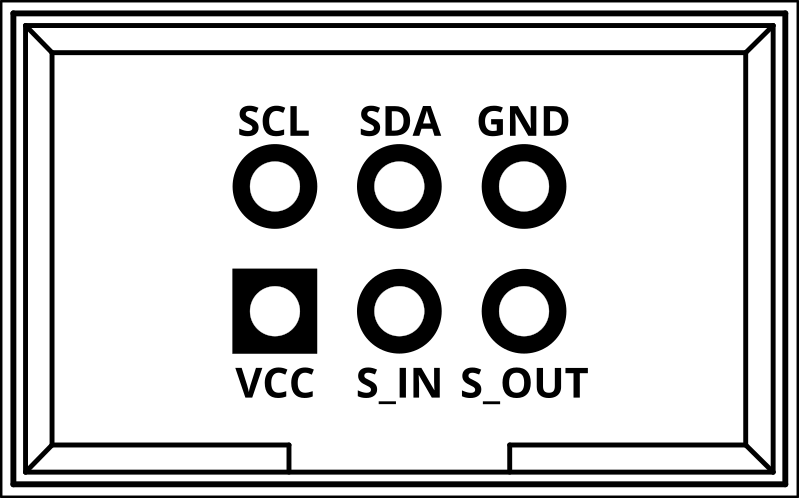
\includegraphics[height=2cm]{2-internal_bus.png}
    \hspace{1cm}
    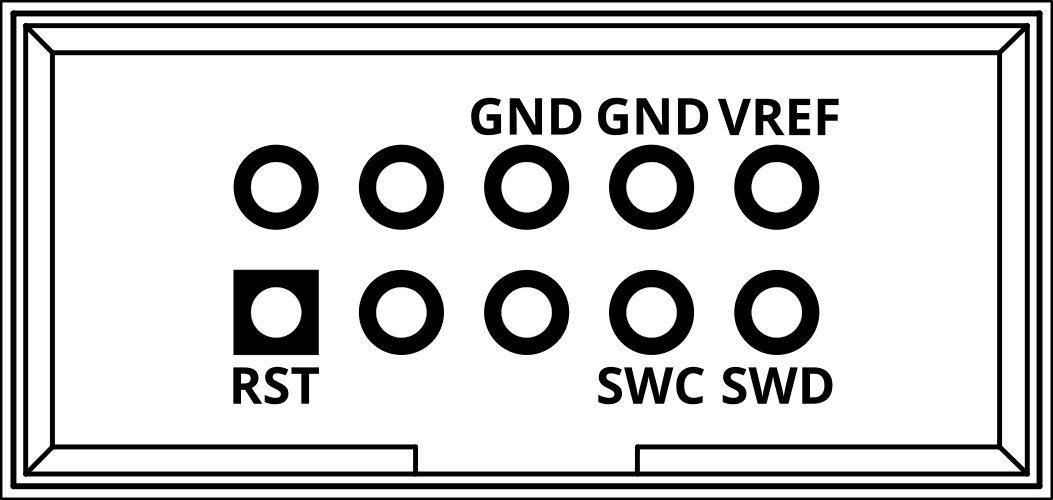
\includegraphics[height=2cm]{2-cortex_debug.png}
  \end{center}
  \caption{Internal communication bus and programming connector layout.}
  \label{fig:connectors}
\end{figure}


To power the microcontroller and because of debugging possibilities, a type B micro \ac{USB} connector was also added to the board. \ac{USB} connection features 2 differential data signals, a $5V$ and ground. Connector additionally has a 'on-the-go' identification pin which is left floating because the requirement does not require a board to become \ac{USB} host. What board implements is a PRTR5V0U2X \ac{ESD} diode\cite{PRTR} which helps protect both the host \ac{PC} and the \ac{PCB} from electrical stress in form of surge or overvoltage.


\section{Component selection and compatibility}

A most important part of the node circuit is a microcontroller. Main requirement for it was the possibility of connecting 16 \ac{ADC} devices without the use of additional \ac{ADC} \ac{IC}. Since other members of \ac{UC-Lab} have experience with programming Atmel microcontrollers, a choice was between ATxmega 8-bit AVR microcontrollers, 32-bit UC3 AVR microcontrollers and Atmel SMART ARM-based \ac{MCU}\footnote{(abbrev. SAM)}. So let's take a look at a sample microcontroller from each of the categories. ATxmega64C3 is a 8-bit AVR microcontroller which features 64KB flash program storage and 4KB of \ac{RAM}, 16 pins provide \ac{ADC} with 12-bit resolution and there is native support for I2C\cite{ATxmega32C3}. AT32UC3C164C is a 32-bit AVR microcontroller with the same flash size and number of 12-bit \ac{ADC} inputs but it features 20KB \ac{RAM}\cite{AT32uc3}. ATSAMD21J16 is a 32-bit ARM based microcontroller which has 8KB \ac{RAM}, 20 \ac{ADC} channels which have programmable gain stage, automatic offset and gain compensation as well as a possibility to oversample the signal to get 16-bit resolution\cite{ATSAMD}. Considering that this microcontroller is cheaper than both AVR microcontrollers and that it supported by multiple third-party frameworks such as ARM mbed, Arduino and Simba, Atmel SAMD was chosen as a microcontroller family that will be used. Atmel SAMD \ac{MCU} family microcontrollers have a naming pattern which makes easy to distinguish chips characteristics. An example will be described on is SAMD21J16B-AU. \textit{SAMD} is product family, \textit{21} is product series, \textit{J} stands for pin count (J = 64pins), \textit{16} is for flash memory density (16 = 64KB), \textit{B} is chip variant, \textit{A} is for package type (A = \ac{TQFP}) and finally \textit{U} is for package grade (U = -40 - 85$^{\circ}$C). A first prototype of the board was developed using ATSAMD21J18-AU which is the same as one found in Atmels SAM D21 Xplained Pro Evaluation Kit but that processors was out of stock when production boards were to be made. This is why ATSAMD21J16-AU, a pin-compatible variant with 64KB instead of 256KB of RAM, was used in production boards. Pin layout of a \ac{TQFP} package can be seen in Figure \ref{fig:pinout}. This pinout is same for all ATSAMD21 microcontrollers with 64-pin \ac{TQFP} package so even smaller memory versions can be used for the cost-saving. 

\begin{figure}[h]
  \begin{center}
    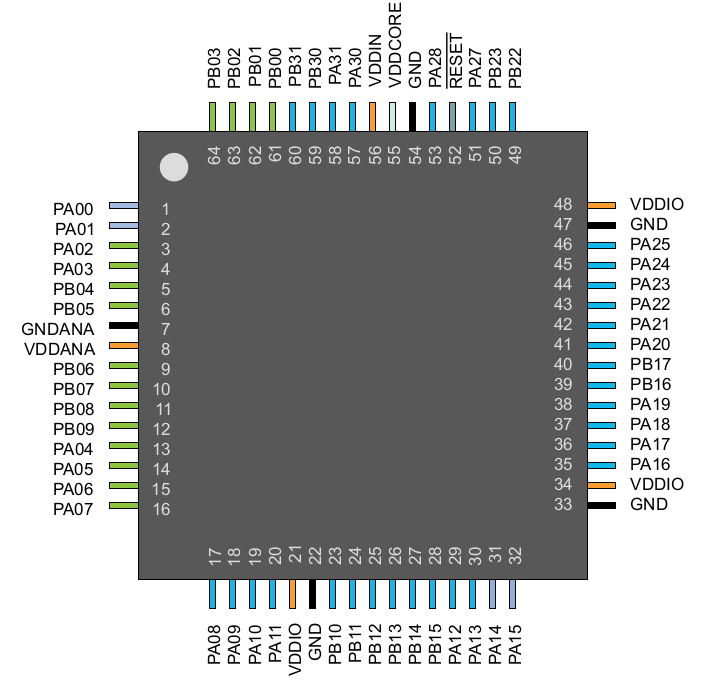
\includegraphics[width=0.4\linewidth]{2-pinout.png}
  \end{center}
  \caption{AT SAMD 64-pin TQFP package pin layout.}
  \label{fig:pinout}
\end{figure}

To power the selected microcontroller a $3.3V$ source is used. Since the most important feature the microcontroller does is analog to digital conversion, it's very important to have a stable and ripple-free \ac{DC} power supply. Oscillations in input voltage to the microcontroller may lead to inconsistent voltage readings. \ac{SMPS} is a very efficient way of \ac{DC}-\ac{DC} conversion but it suffers from a constant high and low frequency voltage ripple. Most of high frequency and some of the low frequency ripple can be countered by using ferrite beads and capacitors but ripple still remains. Breakout board for Intel Edison, an endpoint used in this project, uses TPS62133 $5V$ step-down \ac{SMPS} which can supply a maximum of $3A$ of current\cite{edison_breakout}\cite{TPS6213}. Out of available $15W$, Intel Edison consumes on average $0.41W$ with Wi-Fi enabled. This means that it is possible to use the same power supply for powering the nodes. To filter out the noise a \ac{LDO} is found on each of the nodes. This is in accordance to the specification for high-performance \ac{ADC} power supply design provided by Texas Instruments\cite{SMPS}. \ac{LDO} that was chosen for this project is LD1117 which provides a stable $3.3V$ power supply with $1.1V$ dropout voltage. Input and output voltage lines of the power supply are bridged to the ground with capacitors to filter out the input noise. For debugging a $3.3V$ source can also be attached to ${VREF}$ pin of the programming connector.


\section{PCB design and production}

A \ac{PCB} was designed in KiCad an open-source tool for electronics design automation. First, a microcontroller was placed with decoupling capacitors and ferrite bead according to the manual\cite{ATSAMD}. This ensures low noise during operation. After already described internal bus, programming, sensor and  micro USB connectors were placed, \ac{PCB} was populated with 2 status \ac{LED}s. First \ac{LED} serves as on/off detection and is directly connected to the $V_{cc}$ while the other one is user programmable and can be used for debugging. Board also has a power supply and a reset button. On 3 edges of the board a $3mm$ diameter holes were placed for easy mounting. The layout of the \ac{PCB} can be seen in Figure \ref{fig:pcb_kicad}.

\begin{figure}[h]
  \begin{center}
    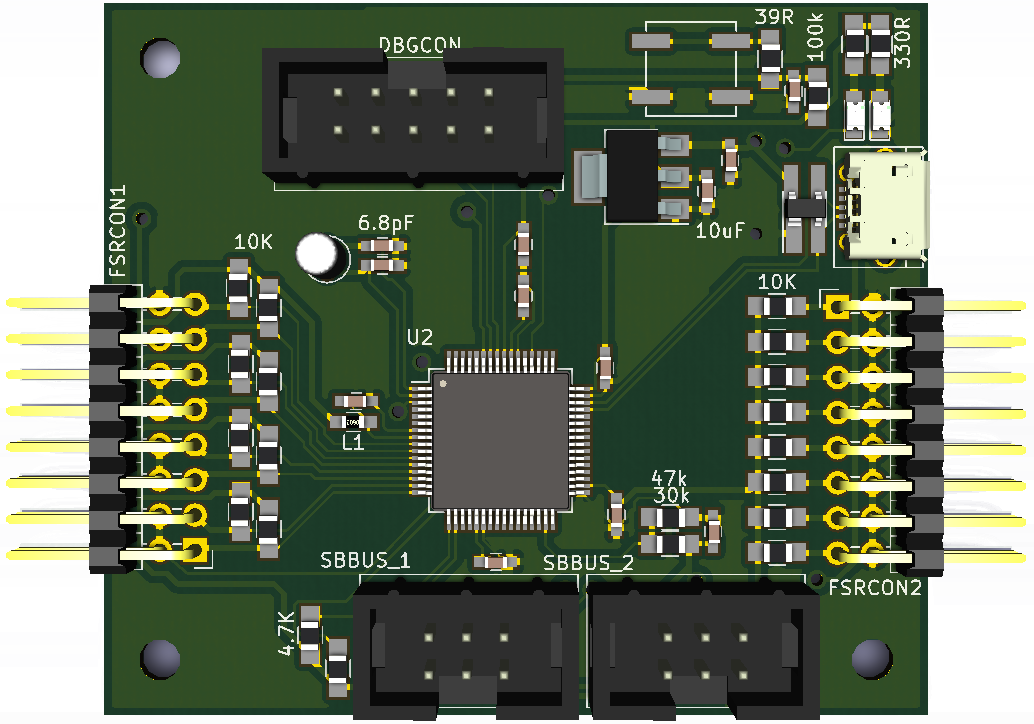
\includegraphics[width=0.45\linewidth]{2-pcb_kicad.png}
    \hspace{1cm}
    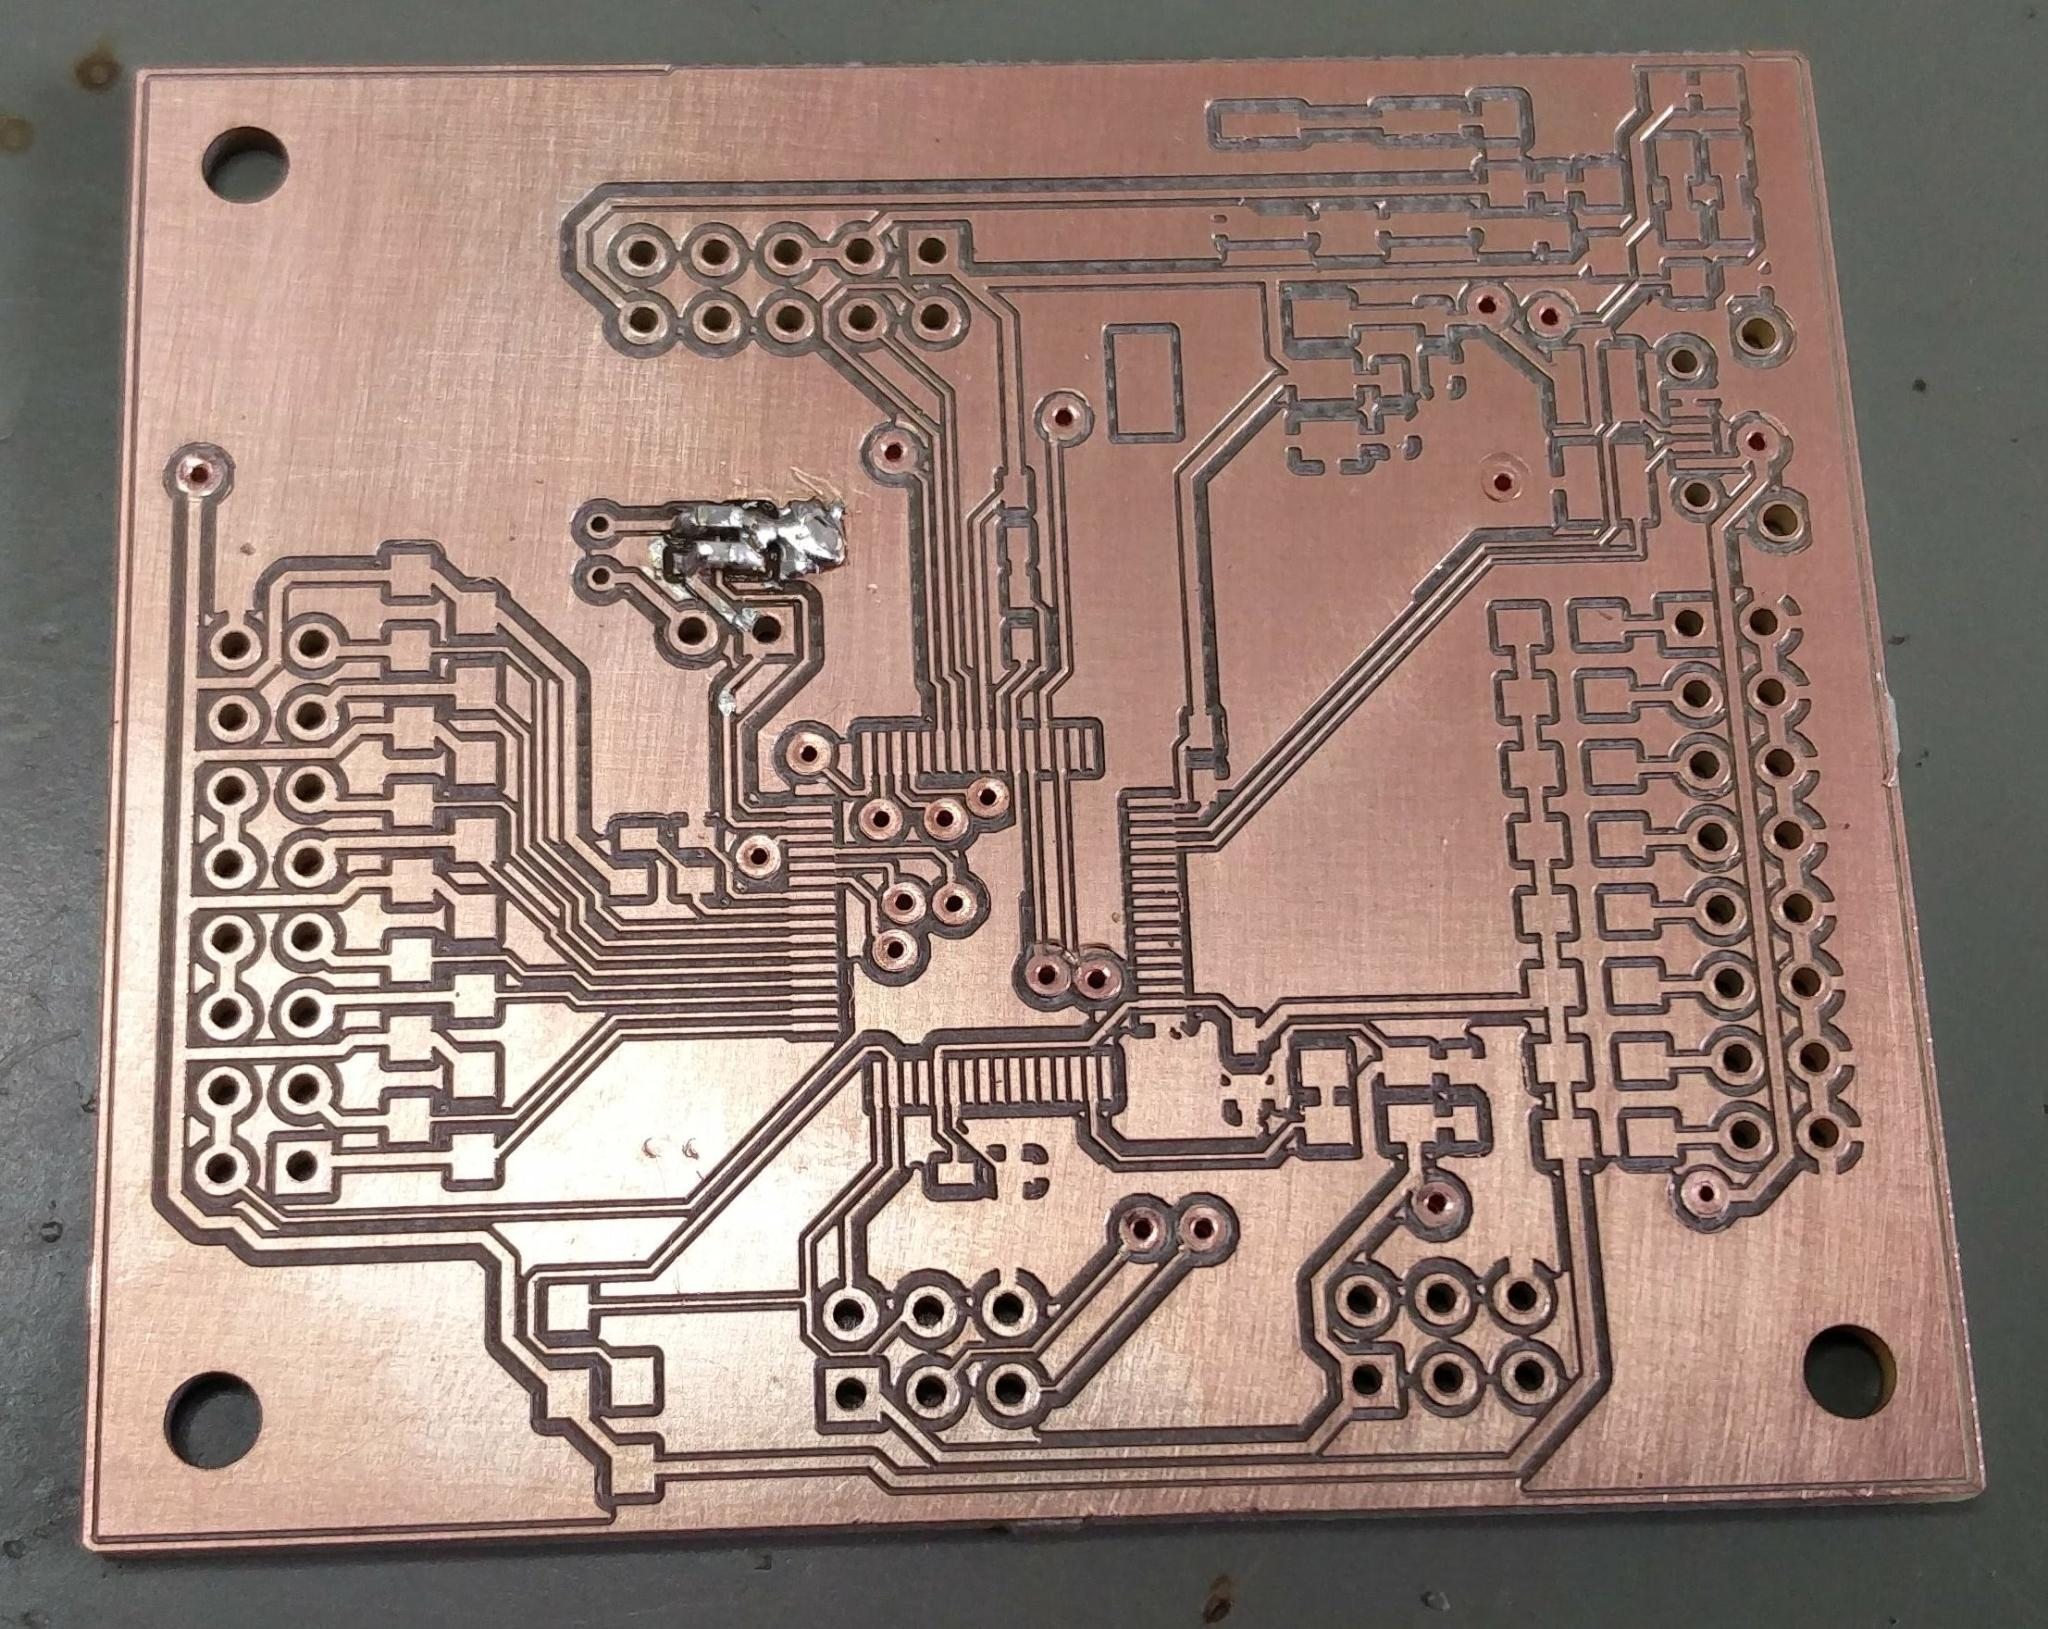
\includegraphics[width=0.4\linewidth]{2-pcb_milled.jpg}
  \end{center}
  \caption{3D view and prototype of printed circuit board developed for the project.}
  \label{fig:pcb_kicad}
\end{figure}

To test the initial design, a board was milled at Department of Electronics at \ac{HTWG} using \href{http://www.lpkf.com/products/rapid-pcb-prototyping/circuit-board-plotter/protomat-s63.htm}{LPKF ProtoMat S63 circuit board plotter}. Since board design features vias, they had to be filled with copper rivets. Prototype production showed that micro USB pin had switched GND and USB OTG ID pins. This error happened due to difference of pin naming between footprint and schematic during the design. After this issue was fixed a board was sent for production to \href{https://aisler.net/}{AISLER}. The components were ordered from DigiKey with already described change from ATSAMD21J18 to ATSAMD21J16. 3 boards were produced and were hand soldered. After production, every board was tested with a sample program reading from each of sensors. The final and assembled board can be seen in Figure \ref{fig:pcb_production}

\begin{figure}[h]
  \begin{center}
    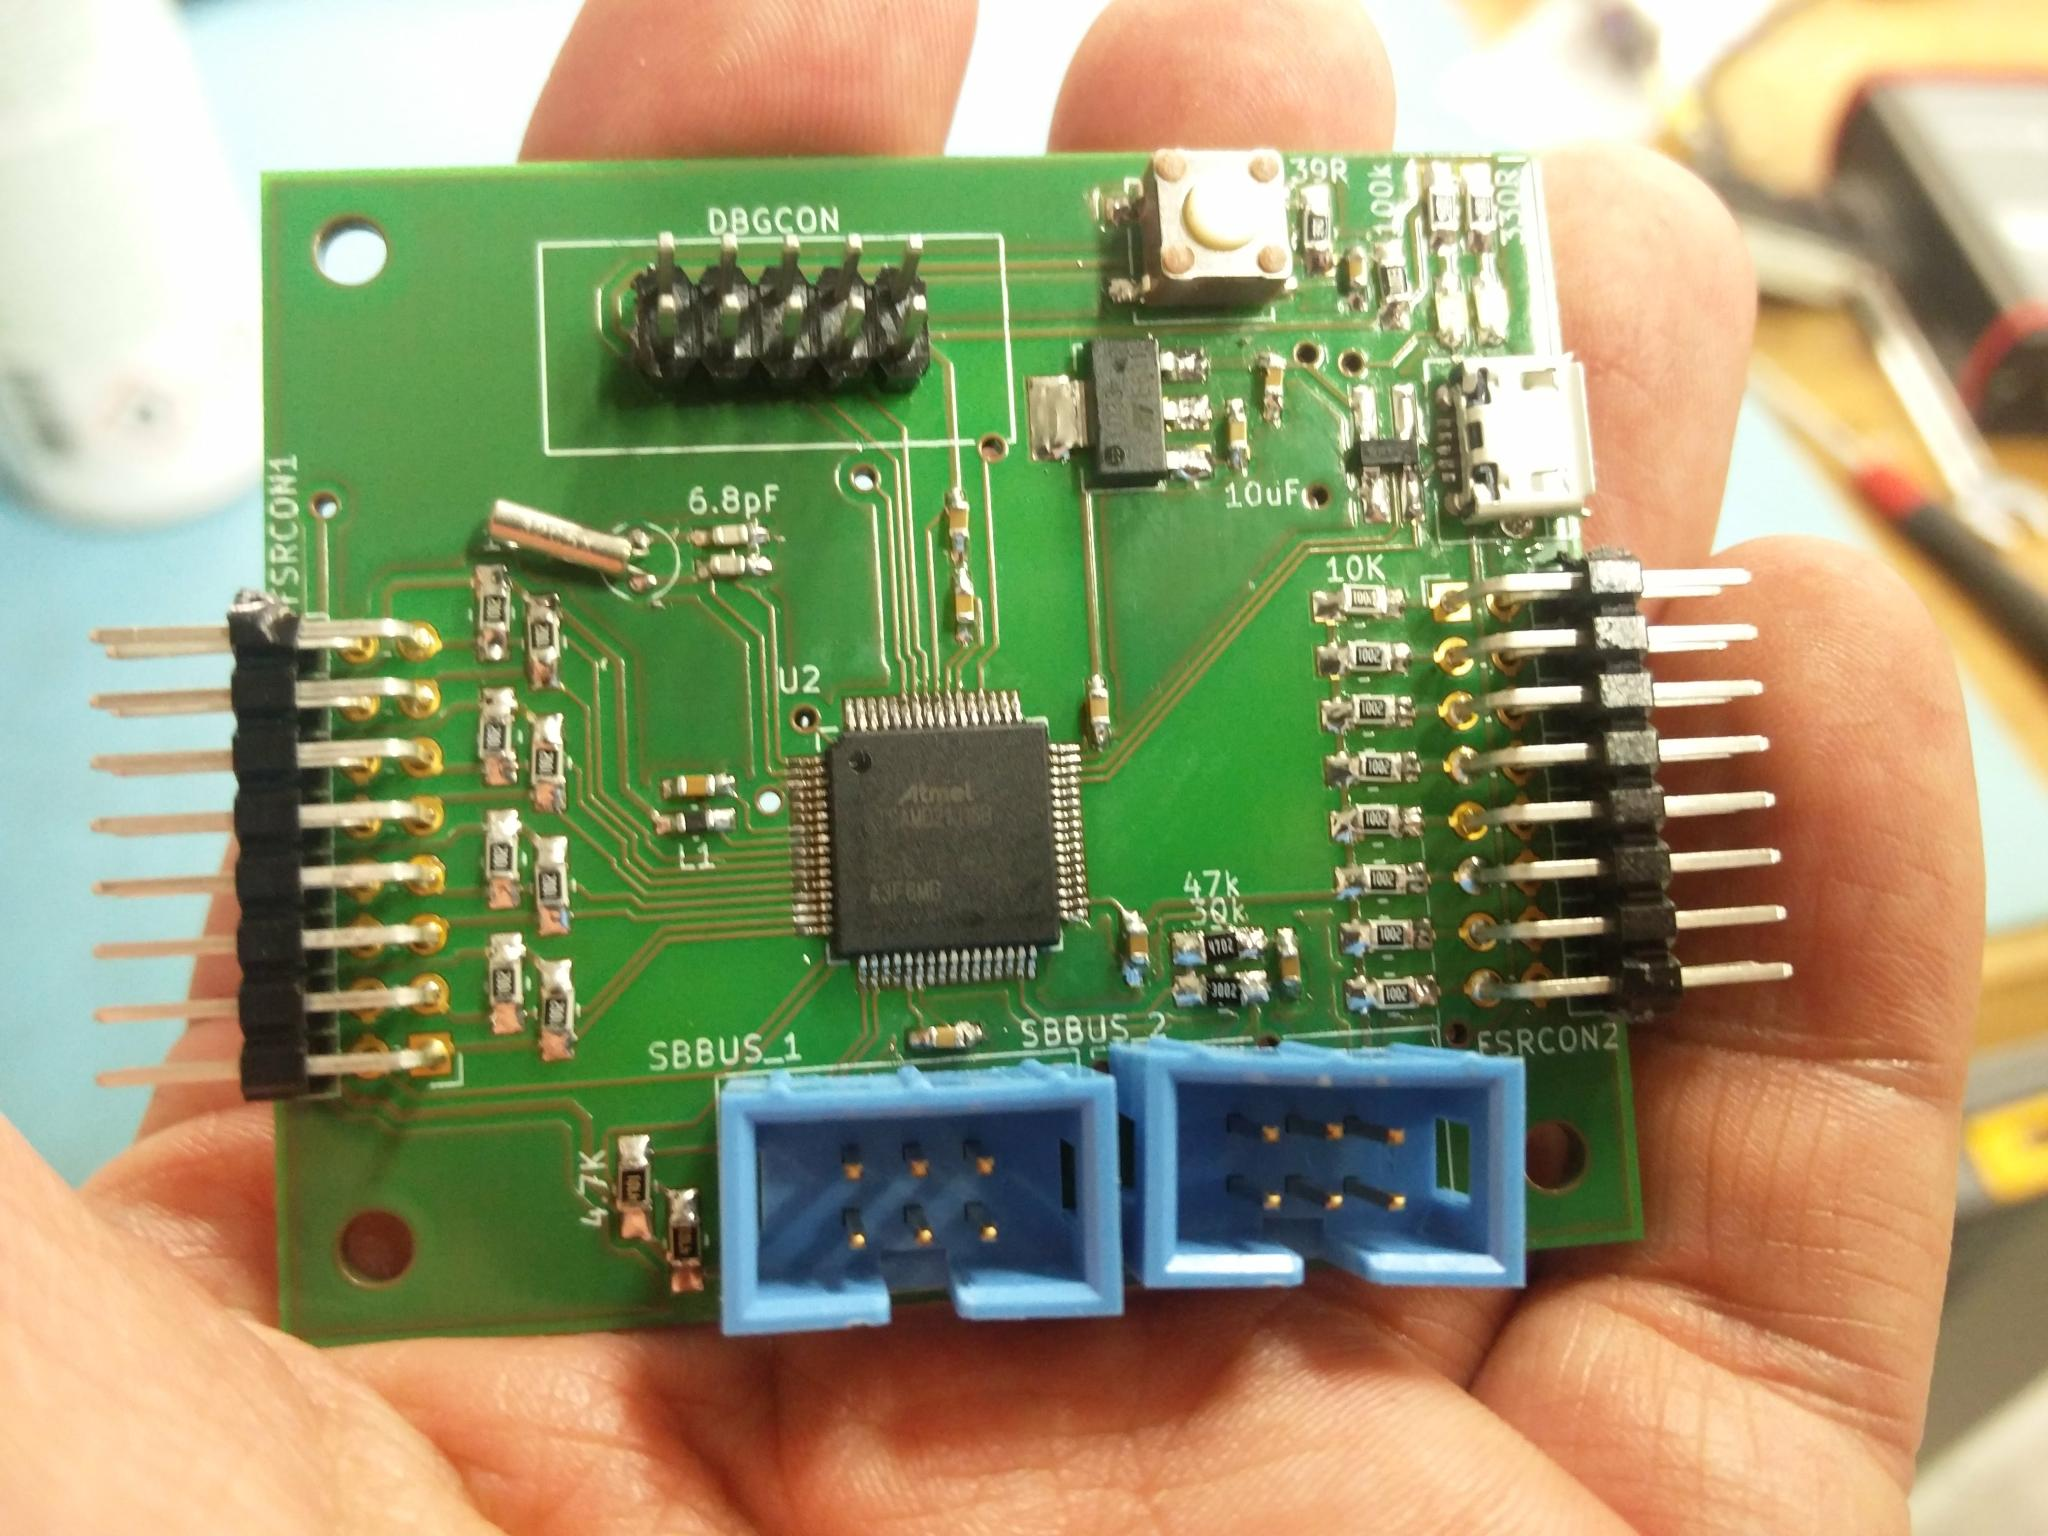
\includegraphics[width=0.45\linewidth]{2-pcb_production.jpg}
  \end{center}
  \caption{Fully populated sensor node circuit board.}
  \label{fig:pcb_production}
\end{figure}


\section{Development environment}

Because of the ARM architecture and Thumb2 instruction set, selected microcontroller supports multiple frameworks and development environments. One of most standardized and widely used frameworks is ARM mbed. It is compatible with almost all ARM microcontroller designs from vendors such as STMicroelectronics, NXP, Renesas, Nordic and Atmel\cite{mbed_devices}. Through abstraction it allows the same code to work on different devices. Depending on the selected device, application code is linked with platform specific libraries and a hex code output file is generated. This hex file can then be uploaded to the microcontroller using "drag and drop" or using \ac{SWD} interface\cite{SWD}. In case of this project, mbed framework was used through \href{http://platformio.org}{Platformio} open source ecosystem for \ac{IoT} development. This environment integrates in Microsoft's VSCode code editor and allows code compiling, upload and debugging along with other features such as intellisense code competition, unit testing and continuous integration. Although both mbed and Platformio support ATSAMD21J18 and Atmels Xplained Pro development board, they provide no support for ATSAMD21J16 variant of the microcontroller. This is why a new configuration for both had to be made.

First, a new board configuration was added to the Platformio configuration folder found in \code{\char`\~/.platformio/boards}. Then a \ac{JSON} structured file was created based upon Atmel Xplained Pro board file but maximum ram size and maximum size were changed because of the smaller \ac{RAM} and flash size. Then a support for a new processor had to be added to the mbed \ac{SDK}. First a new microcontroller and variant were declared an then microcontroller features were described in \code{.platformio/packages/framework-mbed/targets/targets.json}. They can be seen in Listing \ref{lst:mbed_config}. Then, \ac{GPIO} port mapping of this chip variant was declared in \code{port\_api.c}. Next required change included modification of load script. \ac{ROM} was set as rx memory from address 0x00000000 until address 0x00010000 while \ac{RAM} was of rwx type starting from 0x20000000 and with size of 0x2000. Stack size was defined to be 0x500. After these changes were introduced, \ac{BSP} was generated using tool 'tox'. After that, a board became visible in Platformio and programs could be compiled for it.

\begin{lstlisting}[language=json,firstnumber=1,caption={Description of mbed features implemented in ATSAMD21J16},label={lst:mbed_config}]
"SAMD21J16A": {
    "inherits": ["Target"],
    "core": "Cortex-M0+",
    "macros": ["__SAMD21J16A__", "I2C_MASTER_CALLBACK_MODE=true", "EXTINT_CALLBACK_MODE=true", "USART_CALLBACK_MODE=true", "TC_ASYNC=true"],
    "extra_labels": ["Atmel", "SAM_CortexM0P", "SAMD21"],
    "supported_toolchains": ["GCC_ARM", "ARM", "uARM"],
    "device_has": ["ANALOGIN", "ANALOGOUT", "I2C", "I2CSLAVE", "I2C_ASYNCH", "INTERRUPTIN", "PORTIN", "PORTINOUT", "PORTOUT", "PWMOUT", "RTC", "SERIAL", "SERIAL_ASYNCH", "SERIAL_FC", "SLEEP", "SPI", "SPISLAVE", "SPI_ASYNCH"],
    "release_versions": ["2"],
    "device_name": "ATSAMD21J16A"
}
\end{lstlisting}

After program has been compiled and linked for the specific microcontroller, the hex file needs to be uploaded to the microcontroller flash storage. Segger JLink programmer is used for this purpose. To automate the upload a custom script and configuration file were written and integrated into the Platformio. Debugger interface using OpenOCD was also setup so that microcontroller could be debugged from the same development environment.


\section{Software implementation}

A software for the sensor node was written in C++ and compiled using gcc-arm-none-eabi. The main functionalities that were implemented are data readout from sensors and communication with the rest of the system. Each node can be described by the state which is defined by its \ac{I2C} address, sensor state, number of active sensors, with value of each sensor and by currently executing function. To abstract this, a library containing classes used in the project was created. Classes describe data and structures that are used and implement some of the functionality. The rest of the functionality is implemented in main file. It's worth noting that node does not save a longer sensor history but only upon requests serves most recent data.

Class Smartbed is a singleton class which holds state information and provides an easy access to functions regarding the system functionality. Address is a private property of the class and it holds the 7-bit \ac{I2C} address. The address can safely be changed and accessed using mutator methods. Private property \code{active{\_}sensors} saves information which sensors are active in an uint32 data type. For example, if sensor 14 is active, bit 14 is set to 1 while for inactive sensors bits are set to 0. When a change occurs it's considered that sensor is active while an inactive sensor reads the maximum voltage the hole time. Sensor values and pin positions are described in class Sensors which is referenced by Smartbed class. It is also a singleton type and provides methods which access one or all of the sensors and save data in the private property array. Since respiration and hearth pulse are low intensity signals, it is important to have the best possible resolution. Standard resolution of ATSAMD21 \ac{ADC} unit is 12-bit but through the use of subsampling it is possible to get 16-bit resolution which greatly helps in signal recognition.

Two other classes are used for storing temporary communication information. \ac{I2C} packets consist of 7-bit address, read/write flag and data byte or bytes. When a packet is received, an object is created with separated data as a class property. \ac{I2C} also specifies that after every received byte an acknowledgement bit should be set by receiving party. On node side, this is handled by the \ac{I2C} unit of the microcontroller. An endpoint can as a bus master broadcast data using general call address 0, write data to a specific register of the slave or request a read from the device\cite{understanding_i2c}. To distinguish between access types, a class called \code{I2C{\_}RESULT} stores the access type as an enum. This property is set when object is created. Constructor method is overloaded and saves access type depending on the method parameters. If no parameters were supplied, package is invalid and type set to None. If only register address is supplied, master is requesting to read a data from the specified register. If register address and value are supplied master is writing to a register. All of the described classes are shown in Figure \ref{fig:node_classes}.

\begin{figure}[h]
  \begin{center}
    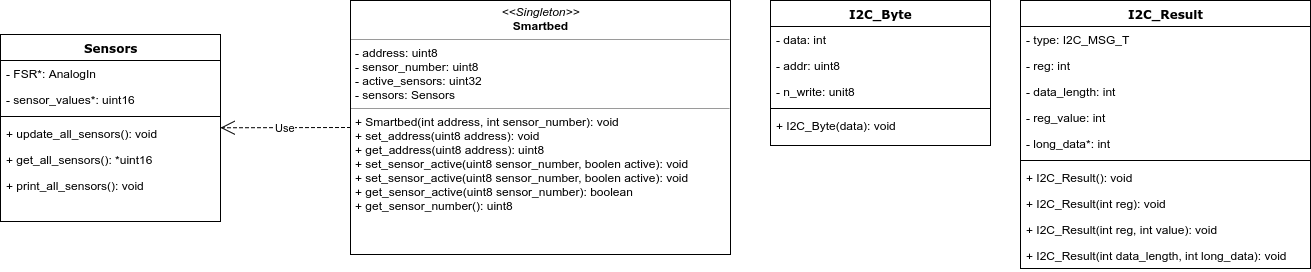
\includegraphics[width=\linewidth]{2-node_classes.png}
  \end{center}
  \caption{Helper classes used in firmware.}
  \label{fig:node_classes}
\end{figure}

The main program starts with the initialization of peripherals - position sensing input pin is set to digital pull down input while and led and position sensing output pin are set as output pins. Then, I2C communication is initialized to operate on $100KHz$ frequency and takes default address 0x10. Since reading subsampled data from \ac{ADC} takes considerable time, reding sensor value after request for its value was requested would result in a timeout. This is why a periodical sensor update is executed roughly every 100ms. Framework's inbuilt Ticker class takes care that function \code{update{\_}all{\_}sensors()} is executed regularly. Unfortunately, mbed does not provide \ac{API} functionality to add custom function as software interrupt when I2C package is received. This is why a main program loop is executing \code{i2c{\_}slave{\_}worker()} function. This function contains main communication logic. It listens to I2C bus and depending on the received data initializes \code{I2C{\_}RESULT} object which is then returned to main function. This object is then transferred to \code{process{\_}i2c{\_}call()} which depending on the message type calls read, write and broadcast (general call) routines. Program logic is visualized in Figure \ref{fig:node_logic}.

\begin{figure}[h]
  \begin{center}
    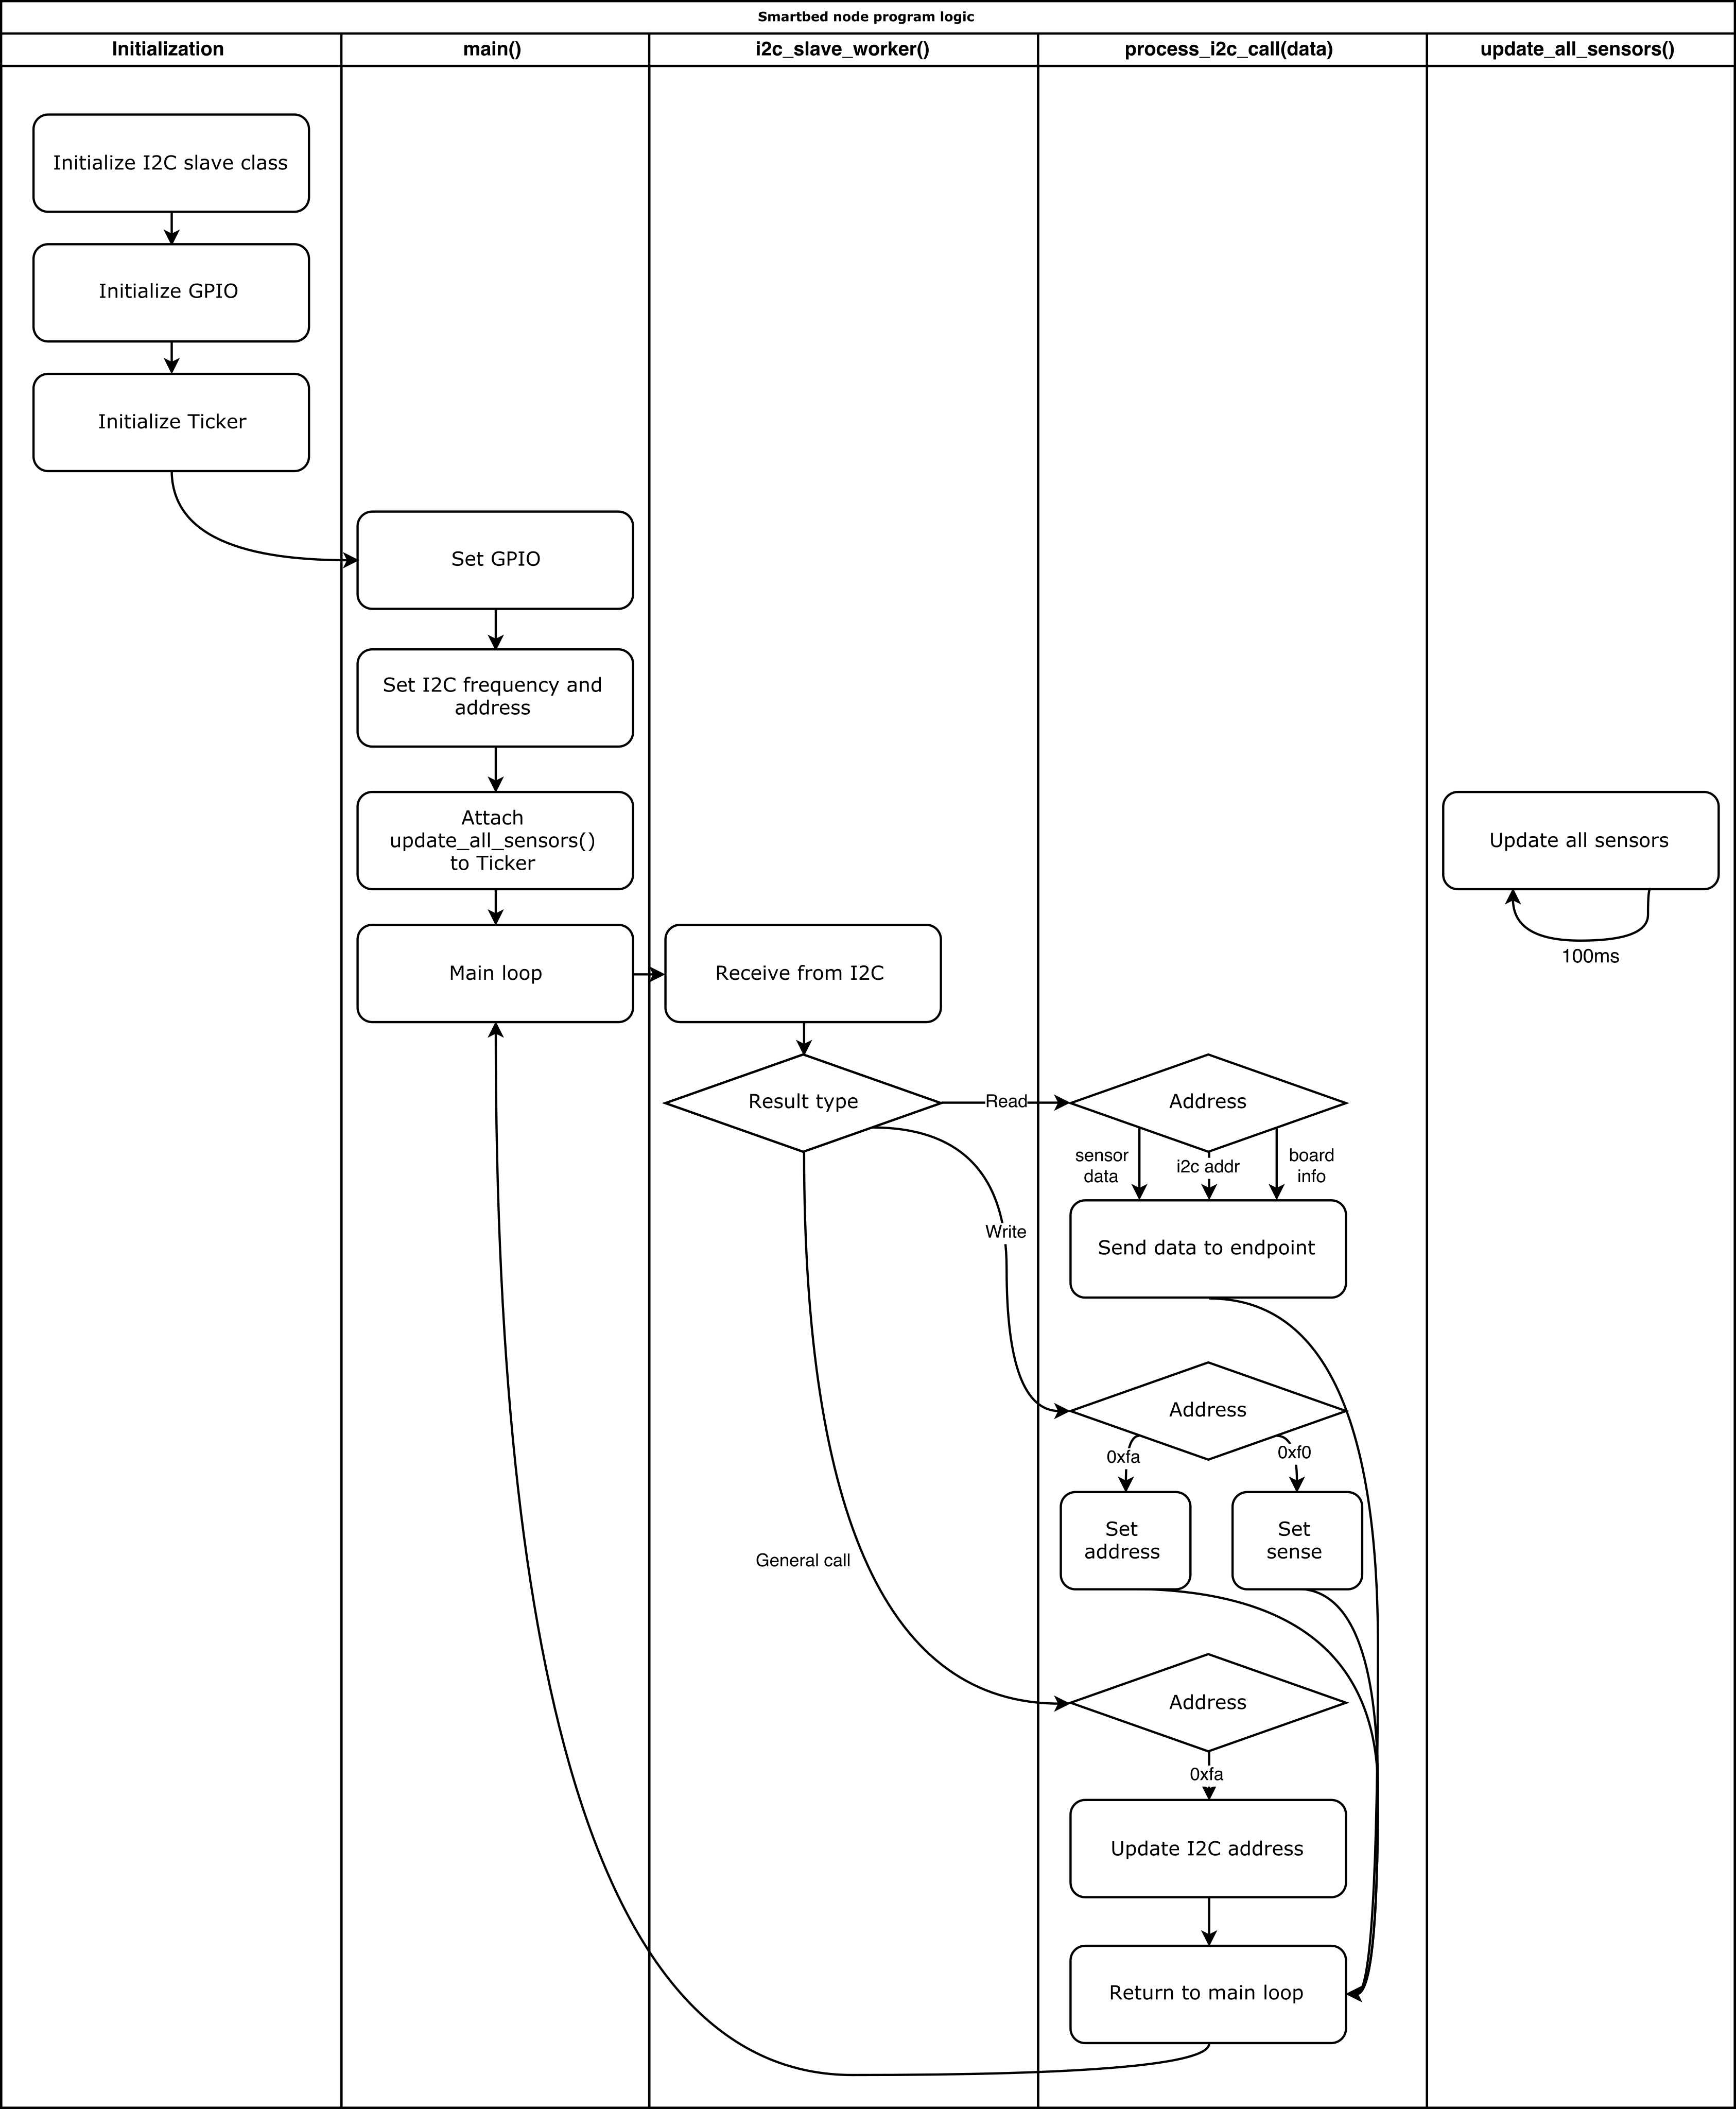
\includegraphics[width=\linewidth]{2-node_logic.png}
  \end{center}
  \caption{Sensor node program flow.}
  \label{fig:node_logic}
\end{figure}

When node is accessed in write mode, two register addresses are writable. Writing a byte to 0xfa will change the address of the node while writing to 0xf0 will set the position sensing output pin high or low depending on the data byte received in the write request. Read requests for registers 0x00 to 0x0f address will return 16-bit value of specified sensor that is stored in \code{Sensors} class. Reading from 0xa0 will return values of all sensors. It's also possible to read from register 0xfa which returns I2C address, from 0xfb which returns number of active sensors, 0xfc returns the board revision which is defined in the header file and 0xfd returns firmware version also found in header file. A read request to all other addresses returns 0xab. When a general call is issued, if register 0xfa is addressed, node will check if position sensing pin is high and change its address to the one in \ac{I2C} package. This enables dynamic configuration of the sensor network and eliminates the need for a different firmware for each board. \\

\begin{table}[h]
  \begin{center}
    \begin{tabular}[h]{ | >{\arraybackslash} m{2.5cm} | >{\arraybackslash} m{2cm} | > {\arraybackslash} m{8cm} |  }
      \hline
      & Register & Description \\ 
      \hline
      Read & 0x00 .. 0x0f & Data for specified sensor (2B) \\ 
      & 0xa0 & All sensor data (32B) \\
      & 0xfa & I2C address (1B) \\
      & 0xfb & Number of active sensors (1B) \\
      & 0xfc & Board revision (1B) \\
      & 0xfd & Firmware version (1B) \\
      & Default & Returns 0xab (1B) \\
      \hline
      Write & 0xfa & Changes node address (1B) \\
      & 0xf0 & Sets position sense sensor value (1B) \\
      \hline
      General call & 0x55 & All nodes reset address to 0x55 (0B) \\
      & 0xfa & If position sense is high, this sensor node takes the supplied address (1B) \\
      \hline
    \end{tabular}
  \end{center}
  \caption{I2C communication interface.}
  \label{tab:i2c_api}
\end{table}

The first node is connected to the endpoint using the system bus cable. The cable attaches to the 6-pin \ac{IDC} connector labeled as \code{SBBUS{\_}1}. To add the second node to the system, a cable needs to connect connector \code{SBBUS{\_}2} on the first node and connector \code{SBBUS{\_}1} on the second node. Difference between this connectors is that pins for \code{SENSE{\_}IN} and \code{SENSE{\_}OUT} are swapped on the \ac{PCB}. This eliminates the need for custom cables or additional resistors. Figure \ref{fig:node_daisychain} demonstrates proper connection of a system containing of an endpoint and 2 nodes. Power can be supplied to the endpoint using microUSB cable.

\begin{figure}[h]
  \begin{center}
    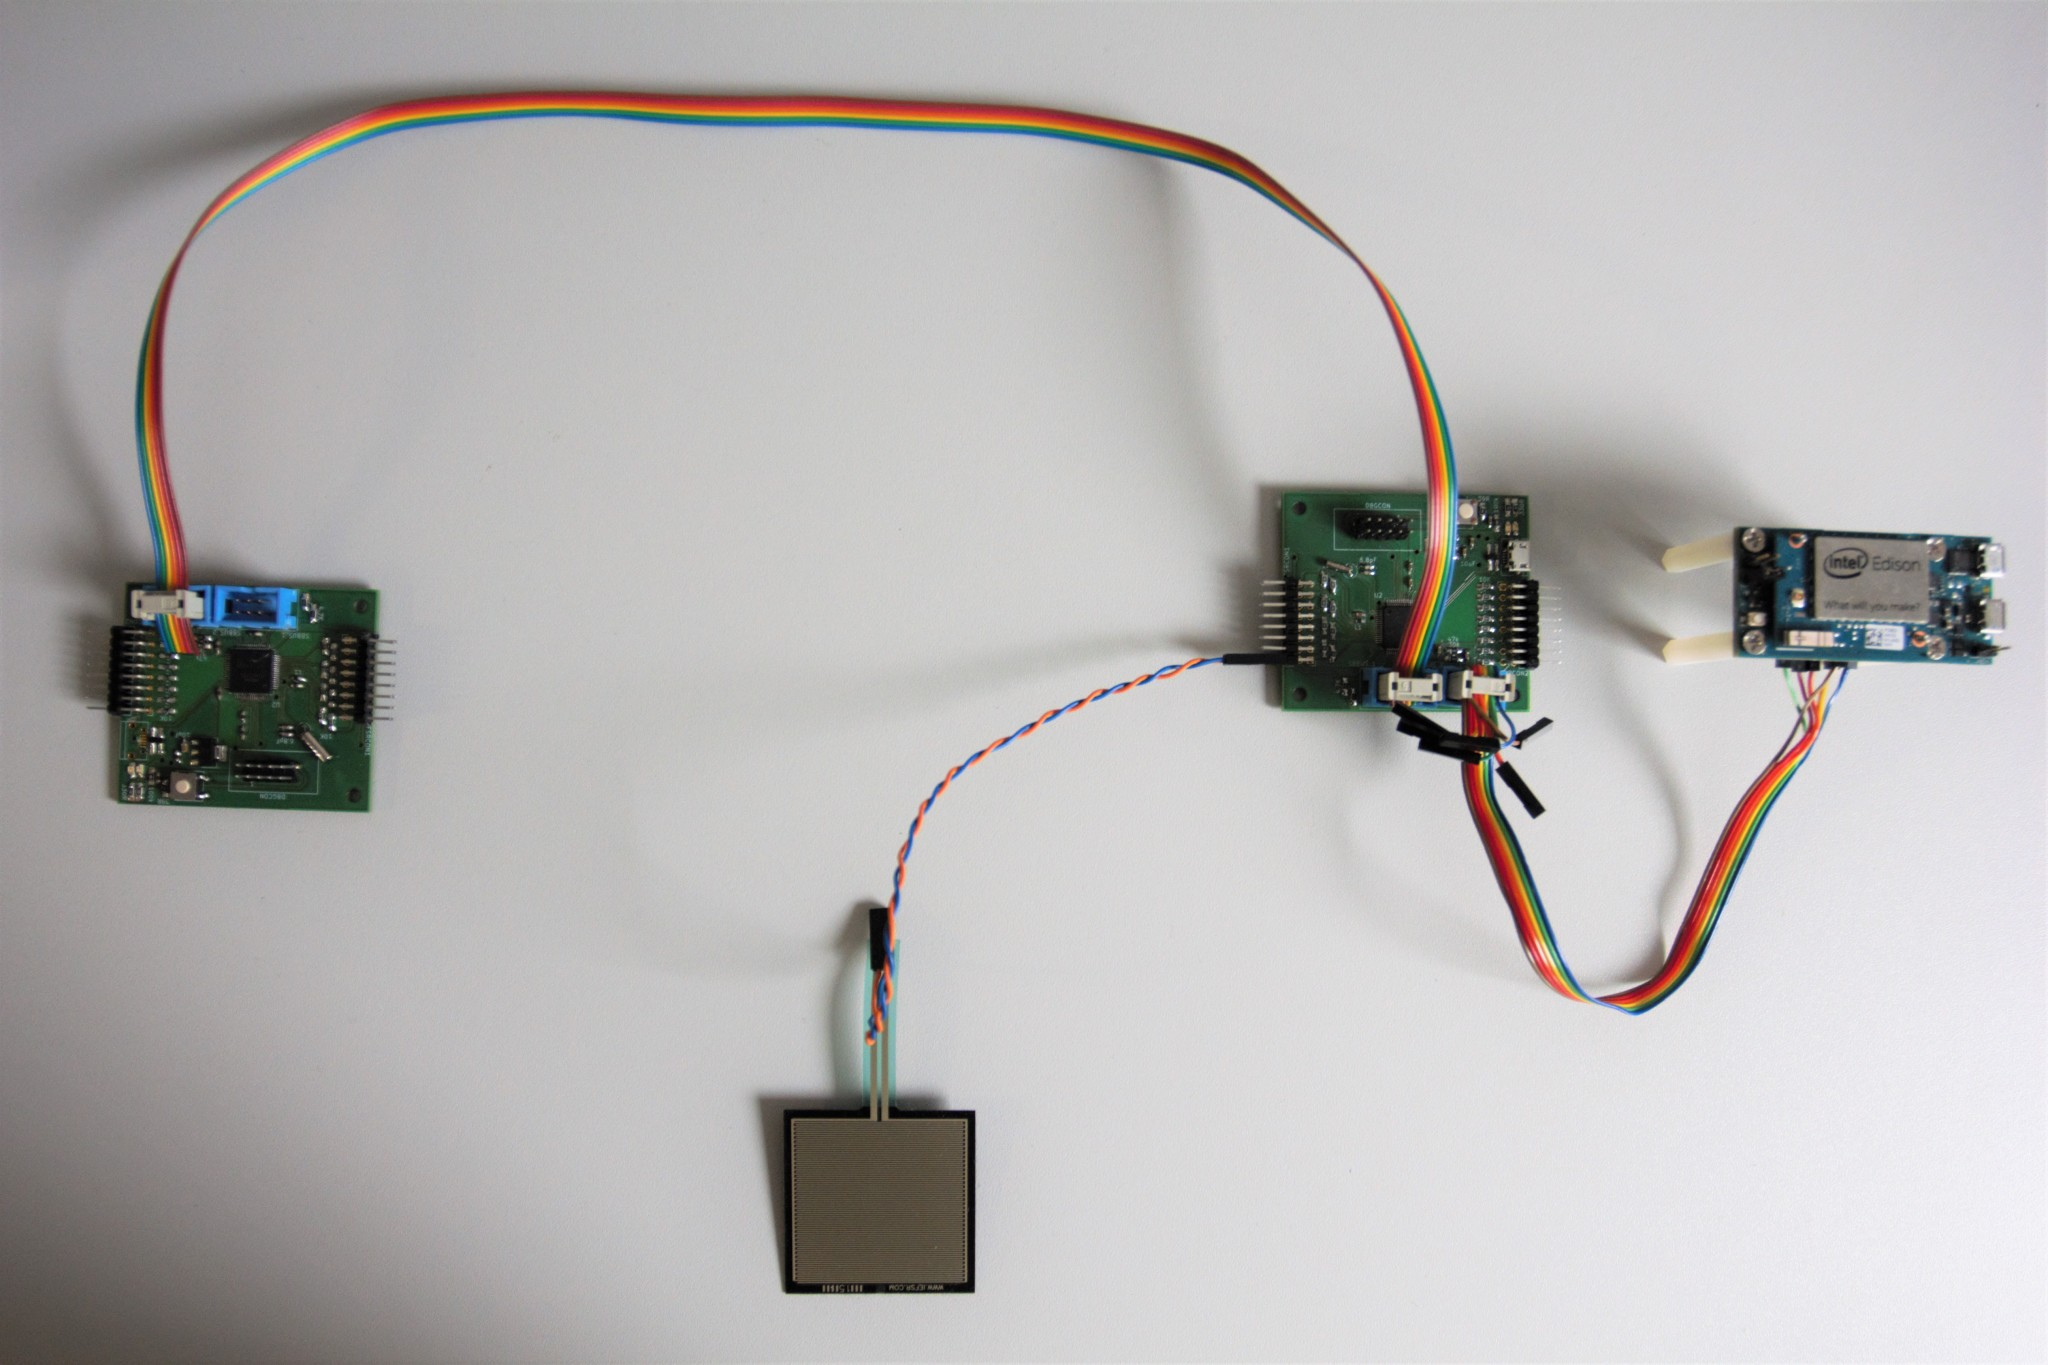
\includegraphics[width=0.65\linewidth]{2-node_daisychain.jpg}
  \end{center}
  \caption{Proper connection of endpoint, two nodes and a FSR sensor.}
  \label{fig:node_daisychain}
\end{figure}